\documentclass[10pt,landscape]{article}
\usepackage{multicol}
\usepackage{calc}
\usepackage{ifthen}
\usepackage[landscape]{geometry}
\usepackage{amsmath,amsthm,amsfonts,amssymb}
\usepackage{color,graphicx,overpic}
\usepackage{bm}
\usepackage{hyperref}



% This sets page margins to .5 inch if using letter paper, and to 1cm
% if using A4 paper. (This probably isn't strictly necessary.)
% If using another size paper, use default 1cm margins.
\ifthenelse{\lengthtest { \paperwidth = 11in}}
    { \geometry{top=1cm,left=1cm,right=1cm,bottom=1cm} }
    {\ifthenelse{ \lengthtest{ \paperwidth = 297mm}}
        {\geometry{top=1cm,left=1cm,right=1cm,bottom=1cm} }
        {\geometry{top=1cm,left=1cm,right=1cm,bottom=1cm} }
    }

% Turn off header and footer
\pagestyle{empty}

% Redefine section commands to use less space
\makeatletter
\renewcommand{\section}{\@startsection{section}{1}{0mm}%
                                {-1ex plus -.5ex minus -.2ex}%
                                {0.5ex plus .2ex}%x
                                {\normalfont\large\bfseries}}
\renewcommand{\subsection}{\@startsection{subsection}{2}{0mm}%
                                {-1explus -.5ex minus -.2ex}%
                                {0.5ex plus .2ex}%
                                {\normalfont\normalsize\bfseries}}
\renewcommand{\subsubsection}{\@startsection{subsubsection}{3}{0mm}%
                                {-1ex plus -.5ex minus -.2ex}%
                                {1ex plus .2ex}%
                                {\normalfont\small\bfseries}}
\makeatother

\newenvironment{lmat}
{\left|\begin{smallmatrix}}
	{\end{smallmatrix}\right|}

\newcommand{\deriv}[1]{\frac{\mathrm{d}}{\mathrm{d}#1} }

% For partial derivatives
\newcommand{\pderiv}[2]{\frac{\partial #1}{\partial #2}}

% Integral dx
\newcommand{\dx}{\mathrm{d}x}
\newcommand{\cd}{\overset{d}{\to}}
\newcommand{\cp}{\overset{p}{\to}}
\newcommand{\B}{\beta}
\newcommand{\e}{\epsilon}
\newcommand{\limn}{\lim_{n\to \infty}}
\newcommand{\lm}{\lambda}
\newcommand{\sg}{\sigma}
\newcommand{\hb}{\hat{\beta}}
\newcommand{\sumn}{\sum_{i=1}^{n}}
\newcommand{\hth}{\hat{\theta}}
\newcommand{\lra}{\Leftrightarrow}
\newcommand{\prodn}{\prod_{i=1}^{n}}
\newcommand{\dll}[1]{\dfrac{\partial\ell}{\partial{#1}}}
\newcommand{\mle}{\hat{\theta}_{MLE}}
\newcommand{\mm}{\hat{\theta}_{MM}}
\newcommand{\sumx}{\sum_{i=1}^{n}x_i}
\newcommand{\ta}{\theta}
\newcommand{\qe}{ \ ?\ }
\newcommand{\dt}{\pderiv{}{\ta}}
\newcommand{\dtt}{\pderiv{^2}{\ta^2}}
\newcommand{\lt}[1]{\log(f(#1|\ta))}
\newcommand{\lx}{\lambda(x)}
\newcommand{\dtau}{\left(\dfrac{d\tau(\ta)}{d \ta}\right)^2}
\newcommand{\samp}{X_1,\dots,X_n \sim}
\newcommand{\ra}{\Rightarrow}
\newcommand{\xxx}{X(X^{\prime}X)^{-1}X^{\prime}}
\newcommand{\xx}{(X^{\prime}X)^{-1}}
\newcommand{\m}{C\xx C^{\prime}}
\newcommand{\p}{\prime}
\newcommand{\hy}{\hat{y}}
\newcommand{\st}{\sg^2}
\newcommand{\sh}{\hat{\sg^2}}
\newcommand{\eh}{\hat{\epsilon}}
\newcommand{\al}{\alpha}
\newcommand{\ga}{\gamma}


\allowdisplaybreaks
% Define BibTeX command
\def\BibTeX{{\rm B\kern-.05em{\sc i\kern-.025em b}\kern-.08em
    T\kern-.1667em\lower.7ex\hbox{E}\kern-.125emX}}

% Don't print section numbers
\setcounter{secnumdepth}{0}


\setlength{\parindent}{0pt}
\setlength{\parskip}{0pt plus 0.5ex}

%My Environments
\newtheorem{example}[section]{Example}
% -----------------------------------------------------------------------

\begin{document}

\raggedright
\footnotesize
\scalebox{0.85}{\begin{tabular}{|c c c c c|}
		\hline
		\textbf{Source of Variation} & \textbf{df} & \textbf{SS} & \textbf{MS} & \boldmath{$F_{obs}$} \\
		\hline
		Intercept & 1 & SSI & SSI & SSI/MSE  \\
		\hline
		Model(uncorrected) & q & USS(model)  & USSM/q & (USSM/q)/MSE   \\
		\hline
		Model(corrected) & q-1 & CSS(model)  & CSSM/q-1 & (CSSM/q-1)/MSE  \\
		\hline
		Error(residual) & N-q & SSE  & SSE/(N-q)=MSE & -  \\
		\hline
		Total(uncorrected) & N & USS(total)  & - & -   \\
		\hline
		Total(corrected) & N-1 & CSS(total)  & - & -  \\
		\hline
\end{tabular}}\scalebox{0.87}{\scalebox{.8}{\begin{tabular}{|c c c |}
	\hline
		T=total & M=Model & E=Error\\
	\hline
		\textbf{Source} & \textbf{Formula} & \textbf{Alternate} \\
		\hline
		CSS(M) & $\sum\hat{y}_i^2 - N\bar{y}^2 = \sum (\hat{y}_i - \bar{y}^2)$ & USS(M) - SSI \\
		\hline
		CSS(T) & $\sum y_i^2 - N\bar{y}^2 = \sum (y_i - \bar{y}^2)$ & USS(T) - SSI \& CSS(M) + SSE\\
		\hline
		CSS(E)/USS(E)/SSE & CSS(T) - CSS(M) & USS(T) - USS(M) = USS(E)\\
		\hline
		SSE & $\sum (\hat{y} - y_i)^2$ & $\sum\hat{\varepsilon}^2$ \\
		\hline
		USS(M) & $\sum\hat{y}_i^2$ & USS(T) - SSE \\
		\hline
		USS(T) & $\sum y_i^2$ & USS(M) + SSE \\
		\hline
\end{tabular} }
\scalebox{.85}{
	\begin{tabular}{|c c c c c |}
	\hline
	\textbf{Source} & \textbf{DF}  & \textbf{Type I SS} & \textbf{MS} & \textbf{F-value} \\
	\hline
	$x_i$ & 1  & Type I SS & T1SS/df = T1SS& MS/MSE(model) \\
	\hline
	& & $\Sigma_{i=1}^{q-1}T1SS_{x_i} = CSS(M)$ &  &   \\
	\hline
\end{tabular} }}\\
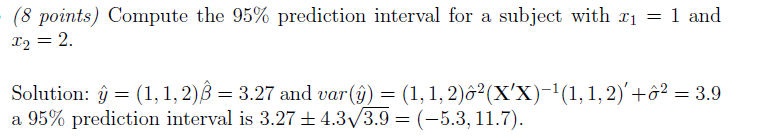
\includegraphics[scale=.6]{fig/pi.png}
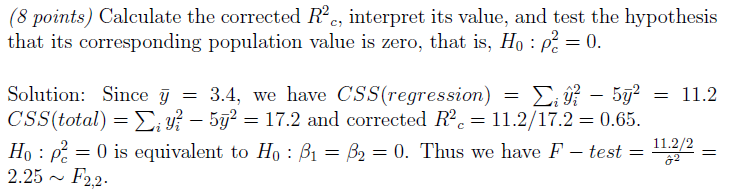
\includegraphics[scale=.6]{fig/rc.png}
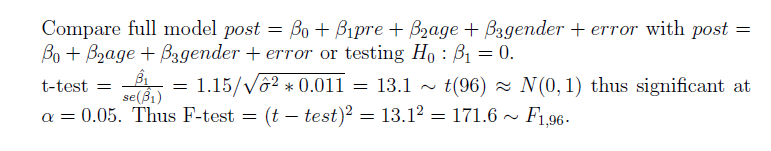
\includegraphics[scale=.6]{fig/mt3.png}
\begin{multicols*}{4}
\setlength{\premulticols}{1pt}
\setlength{\postmulticols}{1pt}
\setlength{\multicolsep}{1pt}
\setlength{\columnsep}{2pt}

% multicol parameters
% These lengths are set only within the two main columns
\setlength{\columnseprule}{.25pt}
\setlength{\premulticols}{.25pt}
\setlength{\postmulticols}{.25pt}
\setlength{\multicolsep}{.25pt}
\setlength{\columnsep}{.25pt}
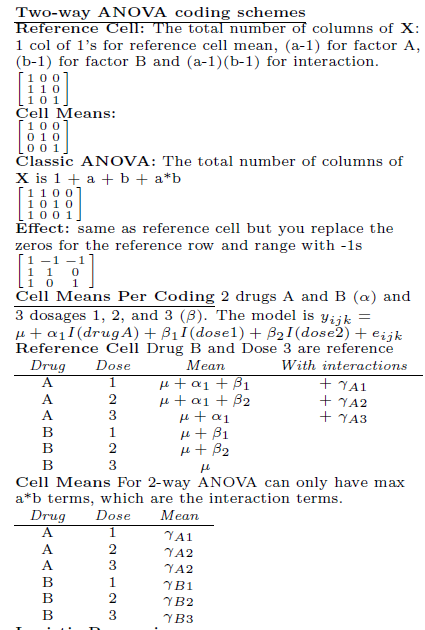
\includegraphics[scale=.55]{fig/2way.png}\\
$(X^{'}X)^{-1}=\begin{lmat}
.308&-.06&-.017\\
-.06&-.025&-.004\\
-.017&-.004&.006
\end{lmat}$ $X^{'}y=\begin{lmat}
405\\1402\\2350
\end{lmat}$\\
\scalebox{.7}{\begin{tabular}{l|l|l|l|l|l}
	\hline
	Source&DF  &SS  & MS  & Fval & $P>F$  \\
	\hline
	Model&2  &79  &239.5  &349.6& $<.001$ \\
	\hline
	Error& 97 & 11  & .113 &  \\
	\hline
	Ctotal&99  &90 &  & \\
	\hline
\end{tabular}}\\
\scalebox{.7}{\begin{tabular}{l|l|l|l|l|l}
	\hline
	param&est  &se  & tval  & $p>|t|$  \\
	\hline
	x0&.67  &.187  &3.58  &.009 \\
	\hline
	x1& 1.35 & .053  & 25.47&$<.001$ \\
	\hline
	x2&1.61  &.026 & 61.81 &$<.001$ \\
	\hline
\end{tabular}}\\
\textbf{2) c)} Test $H_0:\B_1=1$\\
t-test=$\frac{\hb_1-1}{se(\hb_1)}=6.6\sim t_{97}$ $6.6>1.96$ reject $H_0$\\
\textbf{d)} Test $H_0:\B_1=\B_2=1$\\
$B_1=1 \quad B_2=1$ \\
$C=\begin{lmat}
0&1&0\\
0&0&1
\end{lmat}$ $\theta_0=\begin{lmat}
1\\
1
\end{lmat}$ $H_0:C\theta=\theta_0$ $\hat{\theta}=\begin{lmat}
1.35\\
1.61
\end{lmat}$\\
calc M \quad calc $M^{-1}$\\
F-test=$\frac{43.83}{.113}=387.8\sim F_{2,97}$\\
\textbf{e)} 95\% CI of $\B_1+\B_2$ $(\theta)$\\
$\hth=\hb_1+\hb_2=2.96$ $C=[0,1,1]$\\
$se(\hth)=\hat{\sg}^2_{\hth}=\sqrt{.0026}$\\
$2.96\pm 1.96\sqrt{.0026}=[2.86,3.06]$\\
\textbf{f)} Transform $x_1$, $x_2$ to $z_1=x_1-2$, $z_2=x_2-4$\\
Refit with $y^*=\B_0^*+\B_1^*z_1+\B_2^*z_2$\\
$=(\B_0^*-2\B_1^*-4\B_2^*)+\B_1^*x_1+\B_2^*x_2$\\
$\B_0^*=\B_0^*+2\B_1^*+4\B_2^*=9.8$ $C=[1,2,4]$\\
$\sg^2=\hat{\sg}^2C(X^{'}X)^{-1}C^{-1}=.085$ $t=115.3$\\
\textbf{3) f)} is $H_0: \B_0-\B_2=0$ and $\B_1+2\B_2=2$ and $2\B_0+\B_1=2$ testable? Reduce to ETH?\\
$y=\begin{lmat}
0\\2\\3\\6\\10
\end{lmat}$ 
$X=\begin{lmat}
1&6&11\\
1&7&13\\
1&8&15\\
1&9&17\\
1&11&21
\end{lmat}$
$\B=\begin{lmat}
\B_0 \\ \B_1 \\ \B_2
\end{lmat}$\\
$C=\begin{lmat}
1&0&-1\\
0&1&2\\
2&1&0
\end{lmat}$reduces $\begin{lmat}
1&0&-1\\
0&1&2\\
0&0&0
\end{lmat}$ 2pivots $\theta_0=\begin{lmat}
0\\2\\2
\end{lmat}$\\
not FR, not testable, reduces to $C^*$ testable\\
$C^*=\begin{lmat}
1&0&-1\\
0&1&2
\end{lmat}$ $\theta^*_0=
\begin{lmat}
0\\2
\end{lmat}$ $H_0:\begin{lmat}
\B_0-\B_2=0\\
\B_1+2\B_2=2
\end{lmat}$\\
\textbf{1) a)} $x=\begin{lmat}
x_1\\
x_2\\
x_3\\
\end{lmat}\sim N(0,\Sigma)$ $\Sigma=\begin{lmat}
1&0&.6\\
0&1&.5\\
.6&.5&1\\
\end{lmat}$ $c=\begin{lmat}
2 &1 &-1
\end{lmat}$\\
$2x_1+x_2-x_3 \sim N(c\mu,c\Sigma c^{\prime})=N(0,2.6)$ \\
\textbf{b)} $Cov(x_1-x_2,2x_2+x_3)=c_1\Sigma c_2^{\prime}=-1.9$\\
$c_1=\begin{lmat}
1&-1&0
\end{lmat}$ $c_2=\begin{lmat}
0&2&1
\end{lmat}$\\
\textbf{2011 1)} $\hat{\B}=\begin{lmat}
24.877\\
-.231\\
-.185\\
\end{lmat} \quad \hat{\sg^2}=5.59 \ dfE=197$\\ $diag(\xx)=[.03752,.0017,.00056]$\\
$y=\B_0+\B_1x_1+\B_2x_2+\epsilon$\\
$se \B_1=.032 \ \ se \B_2 =.05605$\\
95\% CI $x_1=2 \ x_2=6 \quad C=[1 \ 2 \ 6]$\\
$\hb^*\pm 1.96*se(\hb^*) \quad \hb^*=\hb_0+2\hb_1+6\hb_2=23.3$\\
$se=\sqrt{Var(\hb^*)}=\sqrt{\hat{\sg^2}M}=.1946$\\
Test $H_0:\B_1=3\B_2$ $\ta=\B_1-3\B_2 \ H_0:\ta=0 \ C=[0 \ 1 \ -3]$ 
$t=.327/.1868=1.75\sim t_{97}\approx Z=1.96 \text{ FTR }H_0$\\
Center $x_1 \ x_2$ at means 1,5
$z_1=x_1-1$  $z_2=x_2-5$ $y^*=\B_0^*+\B_1^*z_1+\B_2^*z_2$\\
$\B_0^*+\B_1^*(x_1-1)+\B_2^*(x_2-5)$ $y^*=(\B_0^*-\B_1^*-5\B_2^*)+\B_1^*x_1+B_2^*x_2$\\
$\B_0^*=\B_0+\B_1+5\B_2=-.9116 \ \B_1^*=\B_1 \ \B_2^*=\B_2$\\
$C=[1 \ 1 \ 5] \ se(\B_0^*)=\sqrt{M*\hat{\sg^2}}=.254$\medbreak
\textbf{2)} 4 dose levels (1,2,3,4) 2 methods (oj, aa)\\
n=800 ref cell $\ra$ ref group: aa dose 1\\ $y_i=\mu+\al_1x_{1i}+\al_2x_{2i}+\al_3x_{3i}+\B x_{4i}+\epsilon_i$\\
dummy variables:\\
$x_{1i}=\begin{cases}
1 \text{ if dose=2}\\
0 \text{ otherwise}\\
\end{cases}$ all xs defined similarly\\
$x_{4i}=I(method=oj)$\\
cell mean of each group\\
\scalebox{.8}{ \begin{tabular}{|c c c|}
\hline
Method & Dose & Mean\\
\hline
oj & 1 & $\mu+\B$\\
oj & 2 & $\mu+\al_1+\B$\\
oj & 3 & $\mu+\al_2+\B$\\
oj & 4 & $\mu+\al_3+\B$\\
aa & 1 & $\mu$\\
aa & 2 & $\mu+\al_1$\\
aa & 3 & $\mu+\al_2$\\
aa & 4 & $\mu+\al_3$\\
\hline
\end{tabular}}\\
add interaction btwn method, dose $\ra \ta :8\times 1$\\
let $\mu_o$ and $\mu_a$ be overall means for the two methods\\
write them for models w/ and w/o interaction Derive 2 C matrices for testing $H_0:\mu_o=2\mu_a$ under the 2 models\\
w/o: $\mu_o=\mu+\frac{\al_1+\al_2+\al_3}{4}+\B$  $\mu_a=\mu+\frac{\al_1+\al_2+\al_3}{4}$\\
$H_0:\mu_o=2\mu_a\lra \mu+\frac{\al_1+\al_2+\al_3}{4}-\B=0$\\
$C=(1\ 1/4 \ 1/4 \ 1/4 \-1 )$ for $\ta =(\mu,\al_1,\al_2,\al_3,\B)$\\
w/:$H_0:\mu_o=2\mu_a\lra \mu+\frac{\al_1+\al_2+\al_3}{4}-\frac{\ga_[11]+\ga_{12}+\ga_13}{4}-\B=0$\\
$C=(1\ 1/4 \ 1/4 \ 1/4 \-1 \-1/4 \ -1/4 \ -1/4)$ for $\ta =(\mu,\al_1,\al_2,\al_3,\B,ga_{11},\ga_{12},\ga_{13})$\\
treat dose as a continuous variable and fit model with additive effects of method and dose level with no interaction\\
nested w/in $y_i=\mu+\al_1x_{1i}+\al_2x_{2i}+\al_3x_{3i}+\B x_{4i}+\epsilon_i$? yes\\
write down $H_0$ for comparing the 2 models and derive C
matrix. df of F test under $H_0$?
Let $\al_2=2\al_1$, $\al_3=3\al_1$ (treating dose as continuous)\\
$C=\begin{lmat}
0 & -2 & 1 &0&0\\
0&-3&0&1&0
\end{lmat}$\\
assuming $\ta=(\mu,\al_1,\al_2,\al_3,\B)^{\prime}$\\
df=2 , 7955\\


\textbf{2010 1)} $n=1000$ drugs = A,B doses=1,2,3,4,5\\
ref cell $y=\mu+\alpha_i+\B_{j}+\epsilon$ (w/out interaction)\\
Drug B, Dose 5 ref\\
$\alpha_1$ models effect of drug A\\
$\B_j$ models effect for dose j\\
dims: $y=1000\times 1$ $X=1000\times 6$ $\B=6\times 1$ $\epsilon=1000x1$ $\epsilon\sim N(0,\sg^2I)$\\
Cell mean for each combo of drug and dose:\\
\scalebox{.78}{\begin{tabular}{|c c c|}
\hline
Drug & Dose & Mean\\
\hline
A & 1 & $\mu+\alpha_1+\B_1$\\
A & 2 & $\mu+\alpha_1+\B_2$\\
A & 3 & $\mu+\alpha_1+\B_3$\\
A & 4 & $\mu+\alpha_1+\B_4$\\
A & 5 & $\mu+\alpha_1$\\
B & 1 & $\mu+\B_1$\\
B & 2 & $\mu+\B_2$\\
B & 3 & $\mu+\B_3$\\
B & 4 & $\mu+\B_4$\\
B & 5 & $\mu$\\
\hline
\end{tabular}}\\
for ref cell model p=6 df model $=6-1=5$ \\
with interaction $y_{ijk}=\mu+\alpha_i+\B_j+\gamma_{ij}+\epsilon$\\
$\mu+\alpha_i+\B_4+\B_3+\B_2+\B_1+\gamma{14}+\gamma{13}+\gamma{12}+\gamma{11}+\epsilon$\\
dim ref model: $\B=10\times1$ everything else same\\
\scalebox{.75}{\begin{tabular}{|c c c|}
		\hline
		Drug & Dose & Mean\\
		\hline
		A & 1 & $\mu+\alpha_1+\B_1+\gamma{11}$\\
		A & 2 & $\mu+\alpha_1+\B_2+\gamma{12}$\\
		A & 3 & $\mu+\alpha_1+\B_3+\gamma{13}$\\
		A & 4 & $\mu+\alpha_1+\B_4+\gamma{14}$\\
		A & 5 & $\mu+\alpha_1$\\
		B & 1 & $\mu+\B_1$\\
		B & 2 & $\mu+\B_2$\\
		B & 3 & $\mu+\B_3$\\
		B & 4 & $\mu+\B_4$\\
		B & 5 & $\mu$\\
		\hline
\end{tabular}}\\
$\gamma_{11}$ is the diff btwn the diff of dose1 and dose5 given drug A and b respectively\\
$=[E(y|A,1)-E(y|A,5)]-[E(y|B,1)-E(y|B,5)$\\
Let $\mu_A$ and $\mu_B$ be the overall mean values of cholesterol level for drug A and B\\
$\mu_A=[(\mu+\alpha_1+\B_1+\gamma_{11})+(\mu+\al_1+\B_2+\ga_{12})+(\mu+\al_1+\B_3+\ga_{13})+(\mu+\al_1+\B_4+\ga_{14})+(\mu+\al_1)]/5$\\
$\mu_B=[(\mu+\B_1)+(\mu+\B_2)+(\mu+\B_3)+(\mu+\B_4)+\mu]/5$\\
$H_0:\mu_A=\mu_B\lra H_0\frac{\al_1+\ga_{11}+\ga_{12}+\ga_{13}+\ga_{14}}{5}=0$\\
\textbf{2)} full model in each cell, dose is treated as interval variable\\
$\hat{y}=9.82+3.55*I(drug=A)+2.14 dose+.296age$ $+2.21I(drug=A)* dose+ . 3I (drug =A)*age$\\
fitted model when drug B is used (ref level)\\
$\hat{y}=98.82+2.145dose+2.96age$\\
Write down fitted model when drug A is used\\
$\hat{y}=98.82+3.55*1+2.14dose+.296age+2.21*1*dose+.3*1*age$\\
$\ra\hat{y}=102.37+4.35dose+.596age$\\


\end{multicols*} 
\end{document}